% CVPR 2022 Paper Template
% based on the CVPR template provided by Ming-Ming Cheng (https://github.com/MCG-NKU/CVPR_Template)
% modified and extended by Stefan Roth (stefan.roth@NOSPAMtu-darmstadt.de)

\documentclass[10pt,twocolumn,letterpaper]{article}

%%%%%%%%% PAPER TYPE  - PLEASE UPDATE FOR FINAL VERSION
\usepackage[review]{cvpr}      % To produce the REVIEW version
%\usepackage{cvpr}              % To produce the CAMERA-READY version
%\usepackage[pagenumbers]{cvpr} % To force page numbers, e.g. for an arXiv version

% Include other packages here, before hyperref.
\usepackage{graphicx}
\usepackage{amsmath}
\usepackage{amssymb}
\usepackage{booktabs}


% It is strongly recommended to use hyperref, especially for the review version.
% hyperref with option pagebackref eases the reviewers' job.
% Please disable hyperref *only* if you encounter grave issues, e.g. with the
% file validation for the camera-ready version.
%
% If you comment hyperref and then uncomment it, you should delete
% ReviewTempalte.aux before re-running LaTeX.
% (Or just hit 'q' on the first LaTeX run, let it finish, and you
%  should be clear).
\usepackage[pagebackref,breaklinks,colorlinks]{hyperref}


% Support for easy cross-referencing
\usepackage[capitalize]{cleveref}
\crefname{section}{Sec.}{Secs.}
\Crefname{section}{Section}{Sections}
\Crefname{table}{Table}{Tables}
\crefname{table}{Tab.}{Tabs.}


%%%%%%%%% PAPER ID  - PLEASE UPDATE
\def\cvprPaperID{*****} % *** Enter the CVPR Paper ID here
\def\confName{CVPR}
\def\confYear{2024}


\begin{document}

%%%%%%%%% TITLE - PLEASE UPDATE
\title{Improving Pyramid Scene Parsing Network}

\author{
  Jeongho Son\\
  Department of Computer Science and Engineering, Postech\\
  {\tt\small jeonghoson@postech.ac.kr}
}

\maketitle

%%%%%%%%% ABSTRACT
\begin{abstract}
  Pyramid Scene Parsing network\cite{zhao2017pyramid} is a state-of-the-art semantic segmentation model. The key idea of this model is the Pyramid Pooling Module. The Pyramid Pooling Module calculates the global context of the image, improving the result of ResNet50\cite{he2015deep}. However, some layers of the Pyramid Pooling Module (layer 2, 3, 6) are not utilized well. I address this by changing the structure of the Pyramid Pooling Module. This change adds minimal number of additional parameters.
\end{abstract}

%%%%%%%%% BODY TEXT
\section{Introduction}
\label{sec:intro}

One of the major issues of the ResNet50 based semantic segmentation model is the small receptive field. There are two ways to increasing the receptive field of the ResNet. The first method is to add convolutional layer. The second method is to add a pooling layer. Both methods have disadvantages. The first method increases the number of parameters. The second method reduces the resolution of the feature map. The Pyramid Scene Parsing network\cite{zhao2017pyramid}, one of the state-of-the-art semantic segmentation model, address the receptive field issue using a Pyramid Pooling Module. The Pyramid Pooling Module is a separate module only used to calculate the global context of the image. There are four layers in the Pyramid Pooling Module. I have noticed that three out of four layers are not utilized well. I address this by changing the structure of the Pyramid Pooling Module. This change adds minimal number of additional parameters.

%-------------------------------------------------------------------------
\section{Pyramid Scene Parsing Network}
\label{sec:PSPNet}

\subsection{Receptive Field}
According to the Pyramid Scene Parsing Network paper\cite{zhao2017pyramid}, there are three common issues for semantic segmentation. The issues are mismatched relationship, confusion categories, inconspicuous classes. The main cause of these issues is the small receptive field of the ResNet50\cite{he2015deep}. The model needs to consider global scene context to address the three issues stated above. The small receptive field limits the model's ability to consider global scene context leading to bad performance.

\subsection{Pyramid Pooling Module}
\begin{figure*}[t]
  \centering
  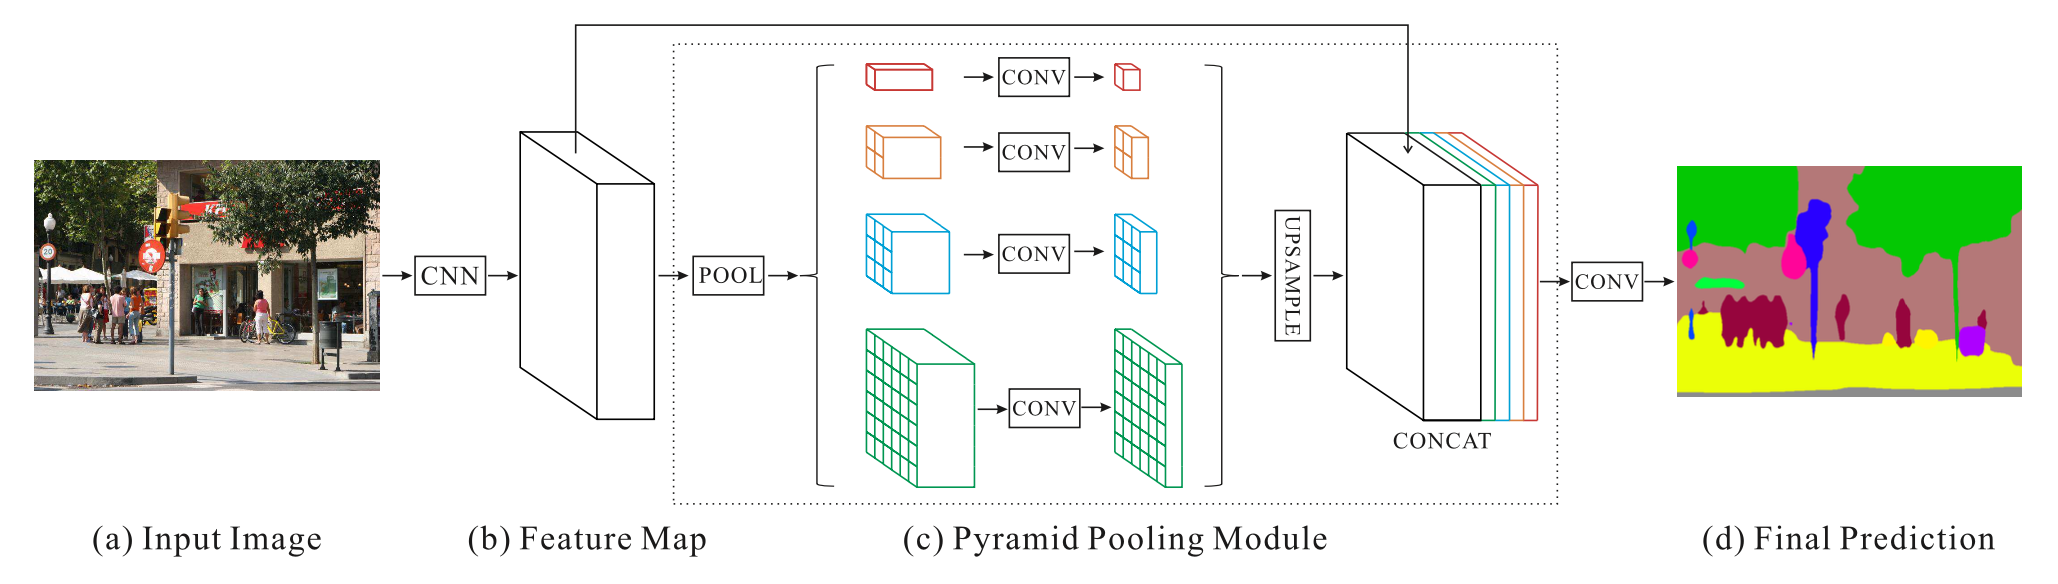
\includegraphics[width=\linewidth]{figures/PSPNet.png}
  \caption{Original PSPNet\cite{zhao2017pyramid} structure.}
  \label{fig:PSPNet}
\end{figure*}
Figure. \ref{fig:PSPNet} shows the original Pyramid Scene Parsing Network structure. The key difference for the Pyramid Scene Parsing Network is the Pyramid Pooling Module. There are multiple layers with different levels, encoding different contexts. The context encoding of the level N layer is as follows. First, the layer divides the image into N x N grid. Each grid is pooled using average pooling. Second, the context of each grid is encoded using a convolution layer with kernel size 1. In other words, there are N x N contexts, each encoding the context of the 1 / (N x N) of the image. Then, each layer is interpolated to the original size and concatenated. For example, the level 1 layer encodes the context of the whole image. The level 2 layer encodes the context of the image divided into 2 x 2 grid. There are level 1, 2, 3, 6 layers in the original Pyramid Pooling Module.

\section{Modified Pyramid Pooling Module}
\label{sec:modified_PSPNet}

\begin{figure*}[t]
  \centering
  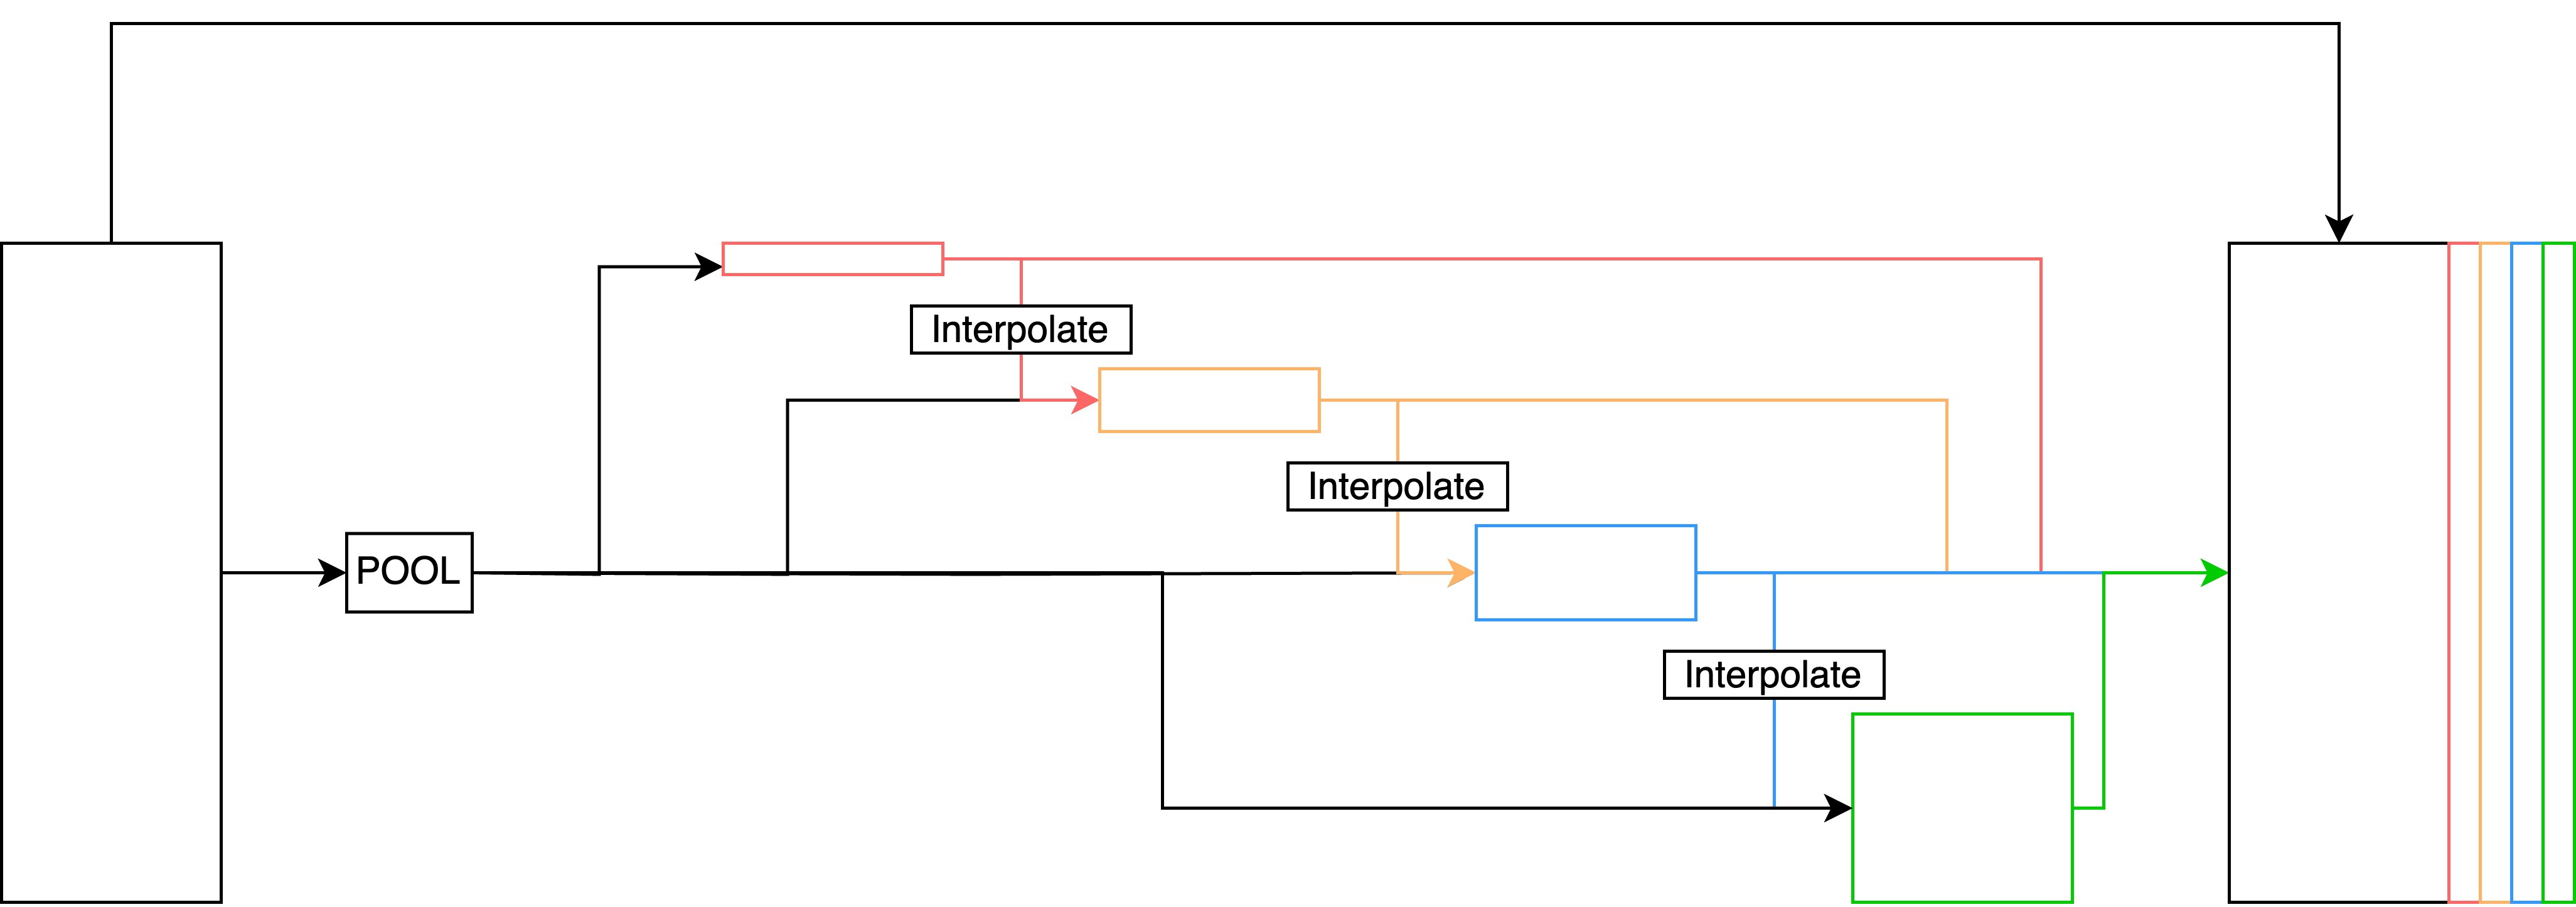
\includegraphics[width=\linewidth]{figures/PSPNet_modified.jpg}
  \caption{Modified PSPNet structure.}
  \label{fig:PSPNet_modified}
\end{figure*}
\begin{figure}[t]
  \centering
  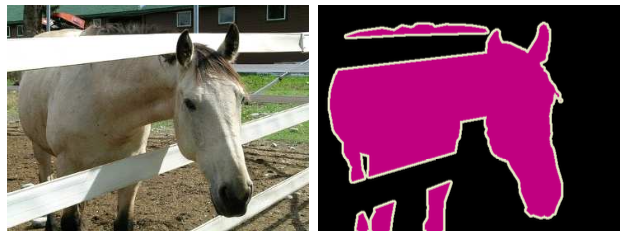
\includegraphics[width=\linewidth]{figures/PASCAL_VOC_horse.png}
  \caption{Example of the PASCAL VOC 2012 image and label.}
  \label{fig:PASCAL_VOC_horse}
\end{figure}
The issue of the original Pyramid Pooling Module is that level N layer only uses 1 / (N x N) of the image to encode the context. For example, level 6 layer will only look at 1 / 36 of the image to encode the context. This means that if there are no objects that are small enough to fit in 1 / 36 of the image, level 6 layer will encode nothing. Consider Figure \ref{fig:PASCAL_VOC_horse}, an example from the dataset PASCAL VOC 2012. In Figure \ref{fig:PASCAL_VOC_horse}, no objects are small enough to know the context by only looking at 1 / 36 of the image. In the PASCAL VOC 2012 dataset, this kind of case is frequent. As a result, while level 1 layer is utilized very well, level 2, 3, 6 layers are not well utilized. I considered this as a problem, and modified the Pyramid Pooling Module to address the issue. My modification allows level 2, 3, 6 layers to be utilized well while the parameter number is approximately the same.

Figure \ref{fig:PSPNet_modified} shows the modification I made. The modification allows level 2, 3, 6 layers to encode the context even if the objects don't fit in the grid. This is done by concatenating context encoding from the previous levels to the input of the next layer.

\section{Experiments}
\label{sec:experiments}

The experiment result is as follows. The baseline model has 57.40\% mean IoU and 66.90\% pixel accuracy. The modified model has 43.79\% mean IoU and 52.36\% pixel accuracy. The training was done using the PASCAL VOC 2012 dataset. I followed the training specifications mention in the original paper\cite{zhao2017pyramid}. The training was done for 50 epochs. The batch size was 2. The model was trained using the PyTorch framework. The model was trained using a single NVIDIA GeForce RTX 3070 GPU.

My modification did not show overall improvement. I think there are two causes for this. First, as I followed the specifications form the original paper, training methods were optimized for the original model. Also, ResNet50, the base of the Scene Parsing Network, was pretrained for the original model. Second, level 2, 3, 6 layers do not need to be fully optimized. The context that does not fit in the grid is already encoded in the previous level. Each level only needs to encode the context that fits in the grid.

However, my model did show improvement for some classes like sofa and tv monitor. As a result, I do not think my modification is completely useless. I think my modification would have produced better results if I used more epochs.

%------------------------------------------------------------------------


%%%%%%%%% REFERENCES
{\small
\bibliographystyle{ieee_fullname}
\bibliography{egbib}
}

\end{document}
